\begin{problem}[21]
调查一下国内做结构物的重力效应实验的离心机有多大, 写出主要参数.
\end{problem}
% --------------------------------------------------------------------

\vspace{10pt}
早在上世纪50年代, 我国在前苏联学术界的影响下开始对离心机的应用有所认识. 到60年代后期, 为研究核能和航空航天技术, 有关部门设计制造了几台大尺寸离心机, 但都为训练飞行人员和检验设备使用. 80年代后各大科研单位和高校开始设计和研制离心模型试验设备, 并应用于解决工程问题\cite{centrifugesParameters}. 经过半个世纪的发展, 应用离心机模拟实验技术在我国已得到广泛应用.

\vspace{-14pt}
\noindent\begin{minipage}[b]{0.55\linewidth}
\indent 如右图所示, 离心机的主要参数为: 有效半径$R$, 最大加速度$g_{\max}$, 最大荷载$m_{\max}$, 模型规模, 容量(单位$gt$, $g$为重力加速度, $t$为质量单位:吨). 表\ref{teb:centrifuges}(见第\pageref{teb:centrifuges}页)列出了截止2011年我国主要离心机及主要参数.
\end{minipage}
\begin{minipage}[b]{0.45\linewidth}
\begin{center}
\usetikzlibrary{%
    decorations.pathreplacing,%
    decorations.pathmorphing,arrows
}


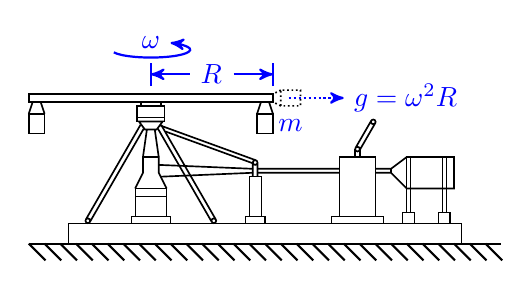
\begin{tikzpicture}[
 interface/.style={
        postaction={draw,decorate,decoration={border,angle=-45,
                    amplitude=0.3cm,segment length=2mm}}}]

\draw[thick,interface] (0,0)--(6,0) ;
\draw (0.5,0.0) rectangle (5.5,0.25)
                                   (1.3,0.25) rectangle (1.8,0.35)
                                   (1.35,0.35) rectangle (1.75,0.6)
                                   (1.35,0.6) rectangle (1.75,0.7)
                                   (2.75,0.25) rectangle (3,0.35)
                                   (2.8,0.35) rectangle (2.95,0.85);

\draw (3.85,0.25) rectangle (4.5,0.35)
             (3.95,0.35) rectangle (4.4,1.1)
             (4.75,0.25) rectangle (4.9,0.4)
             (5.2,0.25) rectangle (5.35,0.4)
             (4.8,0.4) rectangle (4.85,1.1)
             (5.25,0.4) rectangle (5.3,1.1);

\draw[semithick] (4.175,1.2) circle (0.03)
                                  (4.175,1.2) ++(150:0.03)-- ++(60:0.4)
                                  (4.175,1.2) ++(-30:0.03)-- ++(60:0.4)
                                  ++(150:0.03) circle (0.03);
\draw [semithick] (4.145,1.2)--(4.145,1.1)  (4.205,1.2)--(4.205,1.1);

\draw [semithick] (1.65, 1)--(2.85,0.95) (2.85,0.9)--(1.675,0.85)
                                    (2.91,0.95)--(3.95,0.95) (2.91,0.9)--(3.95,0.9)
                                     (4.4,0.95)--(4.6,0.95) (4.4,0.9)--(4.6,0.9)
                                      (4.6,0.9)--(4.6,0.95)--(4.8,1.1)--(5.3,1.1)--(5.4,1.1)--(5.4,0.7)--(4.8,0.7)--cycle;

\draw [semithick] (2.875,1.03)circle(0.03)
                                   (2.845,0.85) --(2.845,1.03) (2.905,0.85)--(2.905,1.03);
\draw [semithick] (2.875,1.03)++(-160:0.03)--++(160:1.18)
                                   (2.875,1.03)++(70:0.03)--++(160:1.3);

\draw[semithick] (1.35,0.7)--(1.45,0.9)--(1.45,1.1)--(1.65,1.1)--(1.65,0.9)--(1.75,0.7)
(1.45,1.1)--(1.5,1.45)--(1.6,1.45)--(1.65,1.1)
(1.5,1.45)--(1.475,1.45)--(1.4,1.55)--(1.7,1.55)--(1.625,1.45)--(1.6,1.45);

\draw[semithick] (1.375,1.55) rectangle (1.725,1.6)
 (1.375,1.6) rectangle (1.725,1.75)
 (1.425,1.75) rectangle (1.675,1.8)
(0,1.8) rectangle(3.1,1.9)
(0,1.4)rectangle (0.2,1.65) 
(2.9,1.4)rectangle (3.1,1.65);
\draw [semithick] (0,1.65)--(0.05,1.8) (0.2,1.65)--(0.15,1.8)
                                    (2.9,1.65)--(2.95,1.8) (3.1,1.65)--(3.05,1.8);
\draw [semithick,densely dotted] (3.2,1.75) rectangle (3.45,1.95) (3.2,1.75)--(3.1,1.8) (3.2,1.95)--(3.1,1.9);

\draw[thick,blue] (1.55,2)--(1.55,2.3) (3.1,2)--(3.1,2.3);
\draw[thick,blue,->,>=stealth'] (2.6,2.15)--(3.1,2.15);
\draw[thick,blue,<-,>=stealth'] (1.55,2.15)--(2.05,2.15) node[right]{$R$};
\draw[blue, thick,->,>=stealth'] (1.55,2.6)++(-160:0.5) arc (-160:60:0.5 and 0.1) node[left]{$\omega$};
\node[blue] at (3.325,1.5) {$m$};
\draw[thick,blue,->,>=stealth',densely dotted] (3.3,1.85)--(4,1.85) node[right]{$g = \omega^2 R$};


\draw[semithick] (0.75,0.29) circle (0.03)
                                  (0.75,0.29) ++(150:0.03)-- ++(60:1.39)
                                  (0.75,0.29) ++(-30:0.03)-- ++(60:1.37);

\draw[semithick] (2.35,0.29) circle (0.03)
                                  (2.35,0.29) ++(210:0.03)-- ++(120:1.37)
                                  (2.35,0.29) ++(30:0.03)-- ++(120:1.39);
\end{tikzpicture}

\end{center}
\end{minipage}


\begin{landscape}
\begin{solution}
\begin{table}[!htb]
\centering
\caption{\label{teb:centrifuges}我国主要离心机及主要技术性能指标\cite{centrifugesParameters}}
{\footnotesize\begin{tabular}{ c c c c c c c c }
\hline 
单位 & 建成时间 & 有效半径/m & 最大加速度/g & 模型规模 & 最大荷载/kg  & 容量/gt & 备注 \tabularnewline
\hline 
中航511厂      & 1960 &6.5 & 80 & 动力 145kW.D.C& 800 & 140 & 飞机工业\tabularnewline
第七机械工业部 &      & 1.7 & 80 & 动力 5kW & 20 &  & 飞机工业\tabularnewline
第二机械工业部 & 1969 & 10.8& 70 & 直径$\times$高度 $0.98 \times 0.88\mathrm{m}$ & 2000 &  & 飞机工业及模拟飞行器\tabularnewline
\hline 
中国工程物理研究院 &  &  &  & 长$\times$宽$\times$高 &  &  & \tabularnewline
第四研究所&1968& 10.8&90 &$0.92\times 0.30\times 0.67 \mathrm{m}$ & 2400 & 216 & 飞机工业及模拟飞行器\tabularnewline
          &1985& 10.8&110&$0.92\times 0.67\times 0.30\mathrm{m}$&3000 & 330 & 主要为军品需求\tabularnewline
\hline 
国防科工委507所&  &  10& 25 &  & 5000 &125 & 模拟飞行器\tabularnewline
华东水利学院(河海大学)&  &2.4&   & $0.48\times 0.28\times 0.15\mathrm{m}$ & 100 & 10 & \tabularnewline
\hline 
                  &1982&2.4&250&$0.90\times0.16\times0.35\mathrm{m}$&100 & 25& \tabularnewline
                  &1982&2.5&300&$0.50\times0.30\times0.15\mathrm{m}$&100 & 20& \tabularnewline
南京水利科学研究院 &    &   &   &$0.45\times0.20\times0.30\mathrm{m}$&    & 30& \tabularnewline
                  &1988&2.1&250&$0.52\times0.40\times0.60\mathrm{m}$&200 & 50& NH-89型\tabularnewline
                  &1992&5.0&200&$1.10\times1.10\times1.10\mathrm{m}$&2000&400& NS-400g\tabularnewline

\hline 
长江水利水电科学院 &1983& 3 &300  &$1.10\times0.33\times0.50\mathrm{m}$&500& 150&\tabularnewline
(长江科学院)       &1983& 3 &300  &$1.10\times0.21\times0.50\mathrm{m}$&10000& 180&\tabularnewline
                  &1985& 3 &300  &$0.76\times0.30\times0.41\mathrm{m}$&1000& 300&\tabularnewline
\hline 
成都勘测设计院 &  & 5 & 200   &  & 1000 & 200 & \tabularnewline
上海铁道学院  &1987&1.55&200 &$0.48\times0.24\times0.32\mathrm{m}$&100&20&L-30型 \tabularnewline
四川(联合)大学  &1990&1.5&250&$0.48\times0.31\times0.30\mathrm{m}$&100&25& \tabularnewline
成都科技大学(今四川大学) &1991&1.54&250 &$0.60\times0.40\times0.40\mathrm{m}$& &25& \tabularnewline
中国水利水电科学研究院  &1993 &4& 300 &$1.50\times1.00\times1.50\mathrm{m}$& & 450&LXJ-4-450 \tabularnewline
  &  &   &    & & &50 & NS-89型\tabularnewline
清华大学  &1993& 2&200&$0.75\times0.50\times0.60\mathrm{m}$&250&50&TH-50gt, 拟静力\tabularnewline
          &  &   &    &$0.50\times0.20\times0.30\mathrm{m}$& &  &动力固壁式\tabularnewline
          &  &   &    &$0.50\times 0.20\times 0.35\mathrm{m}$& &  & 动力叠环式\tabularnewline

香港科技大学&1997&4.5 & 150&$ 1.50\times1.50\times1.60\mathrm{m}$&2670 & 400 &拟静力 \tabularnewline
           &    &    &  75&$ 0.60\times0.60 \times0.4 \mathrm{m}$& &  & 动力\tabularnewline
西南交通大学&2002&2.7&200&$0.60\times 0.40\times0.40\mathrm{m}$&500&100& \tabularnewline
重庆交通大学&2005& 2 &200&$0.70\times0.60\times0.40\mathrm{m}$&300&60& \tabularnewline
长安大学    &2005& 2 &200&$0.60\times0.36\times0.50\mathrm{m}$&300&60& \tabularnewline
同济大学    &2005& 3 &200&$0.70\times0.70\times0.90\mathrm{m}$&750&150&安装机械手\tabularnewline
\hline 

\end{tabular}}
\end{table}
\textcolor{red}{谈老师批注: ``第二机械工业部''和``中国工程物理研究院''为同一单位.} 经本人核实\cite{caep}, 确实如此.
\end{solution}
\end{landscape}
